\documentclass[tikz,border=8pt]{standalone}
\usepackage{ctex,amsmath}
\usetikzlibrary{arrows.meta,positioning}
\usepackage{../../my-math}
\begin{document}
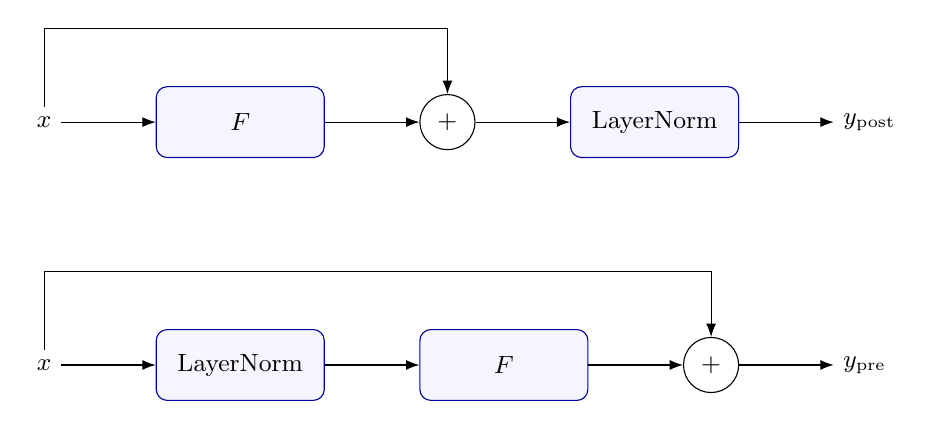
\begin{tikzpicture}[>=Latex,font=\small,node distance=12mm,
 box/.style={draw=blue!60!black,fill=blue!4,rounded corners,align=center,minimum height=9mm,text width=19mm},
 sum/.style={draw,circle,minimum size=7mm}]
\node (x) {$\vect{x}$};\node[box,right=of x] (f) {$F$};\node[sum,right=of f] (add) {$+$};\node[box,right=of add] (norm) {LayerNorm};\node[right=of norm] (out) {$\vect{y}_{\mathrm{post}}$};
\draw[->] (x)--(f);\draw[->] (f)--(add);\draw[->] (add)--(norm);\draw[->] (norm)--(out);
\draw[->] (x.north)--++(0,10mm)-|(add.north);
\node[below=27mm of x] (px) {$\vect{x}$};\node[box,right=of px] (pn) {LayerNorm};\node[box,right=of pn] (pf) {$F$};\node[sum,right=of pf] (pa) {$+$};\node[right=of pa] (po) {$\vect{y}_{\mathrm{pre}}$};
\draw[->] (px)--(pn);\draw[->] (pn)--(pf);\draw[->] (pf)--(pa);\draw[->] (pa)--(po);
\draw[->] (px.north)--++(0,10mm)-|(pa.north);
\end{tikzpicture}
\end{document}
